\begin{task}{340}
Докажите, что если $||G|| = \left\lfloor n^2/4\right\rfloor +1$, то в графе $G$ есть по крайней мере $\left\lfloor n/2\right\rfloor $ треугольников.
\end{task}

\begin{solution}
Докажем индукцией по $n$:\par
\underline{База:}\par
\begin{enumerate}
      \item $|E| = \left\lfloor 1/4\right\rfloor  + 1 = 1$ и \exists \ $\left\lfloor 1/2\right\rfloor  = 0$ треугольников. Очевидно, верно.
    \item $|E| = \left\lfloor 4/4\right\rfloor  + 1 = 2$ и \exists \ $\left\lfloor 2/2\right\rfloor  = 1$ треугольник. Графа с таким количеством ребер на двух вершинах не существует, поэтому посылка не выполнена.
    \item $|E| = \left\lfloor 9/4\right\rfloor  + 1 = 3$ и \exists \ $\left\lfloor 3/2\right\rfloor  = 1$ треугольник. Очевидно, верно.
    \item $|E| = \left\lfloor 16/4\right\rfloor  + 1 = 5$ и \exists \ $\left\lfloor 4/2\right\rfloor  = 2$ треугольника. Очевидно, верно (почти полный граф на четырех вершинах, без одного ребра).
    \item $|E| = \left\lfloor 25/4\right\rfloor  + 1 = 7$ и \exists \ $\left\lfloor 5/2\right\rfloor  = 2$ треугольника. Очевидно, верно (просто добавим одну вершину и два любых ребра к предыдущему графу, то есть у графов на пяти вершинах с таким числом ребер есть подграф на четырех вершинах, изоморфный рассмотренному ранее).
\end{enumerate}

\underline{Переход:}\par Разберем несколько случаев.
\begin{enumerate}
    \item Все ребра лежат в каком-то треугольнике.\par
    Рассмотрим индикаторы: $\operatorname{I}(e \in t)$, где $e$ ---     какое-то ребро, а $t$ --- какой-то треугольник. Очевидно,     $\sum_{e \in E} \sum_{t\in T} \operatorname{I}(e \in t) \geq     |E|$, так как каждое ребро лежит хотя бы в одном треугольнике.     С другой стороны, $\sum_{t \in T} \sum_{e\in E}     \operatorname{I}(e \in t) = 3|T|$. Имеем $3|T|\geq|E|$, или     $3|T|\geq \left(\left\lfloor \frac{n^2}{4}\right\rfloor  + 1\right)$.\par
    Нужно доказать неравенство $3\left\lfloor \frac{n}{2}\right\rfloor  \leq     \left(\left\lfloor \frac{n^2}{4}\right\rfloor  + 1\right)$, при $n \geq 6$.
    Очевидно: \\ $3\cdot\left\lfloor \frac{n}{2}\right\rfloor  \leq {\left\lfloor \frac{n}{2}\right\rfloor }^2$, при $n     \geq 6$. Учитывая $\left\lfloor \frac{n^2}{4}\right\rfloor  + 1\geq {\left\lfloor \frac{n}{2}\right\rfloor }^2$, получим  $3\cdot\left\lfloor \frac{n}{2}\right\rfloor  \leq {\left\lfloor \frac{n}{2}\right\rfloor }^2 \leq     \left\lfloor \frac{n^2}{4}\right\rfloor  + 1$.\par
    Получим: $3|T| \geq \left\lfloor \frac{n}{2}\right\rfloor ^2 \geq 3\left\lfloor \frac{n}{2}\right\rfloor $ при $n     \geq 6$. Имеем $|T| \geq \left\lfloor \frac{n}{2}\right\rfloor $.
    
    \item \exists \ ребро $\{A,B\}$, не лежащее ни в одном треугольнике. Отсюда следует, что суммарно из двух вершин в остальную часть графа выходит не более $n-2$ ребер.
        \begin{enumerate}
            \item Пусть из $A$ и $B$ идет в совокупности $n - 2$ ребра в оставшуюся часть графа. В $G'$ (оставшийся     граф) --- $|E'| = \left\lfloor \frac{n^2}{4}\right\rfloor  + 1 - n + 1$. Так как     для $G'$ выполнено предположение индукции --- в $G'$     есть хотя бы $\left\lfloor \frac{n - 2}{2}\right\rfloor  = \left\lfloor \frac{n}{2} - 1\right\rfloor $ треугольник. Надо найти еще один треугольник, не     лежащий в $G'$, но лежащий в $G$. Сделать это можно, использовав принцип Дирихле. Достаточно заметить, что две из трех вершин какого-то треугольника будут соединены с  $A$ или $B$. В конечном графе могут быть такие картинки:
            \begin{figure}[H]
              \centering
              \begin{subfigure}[a]{0.24\linewidth}
                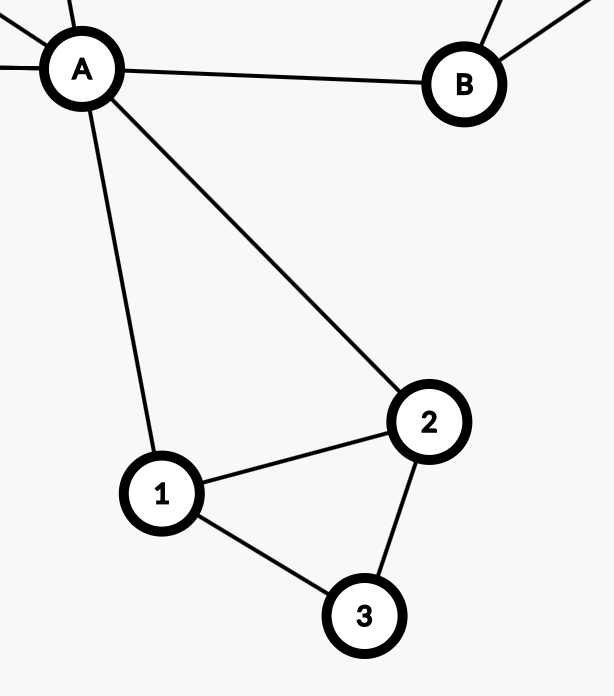
\includegraphics[width=\linewidth]{_img/340/01.png}
              \end{subfigure}
              \begin{subfigure}[a]{0.24\linewidth}
                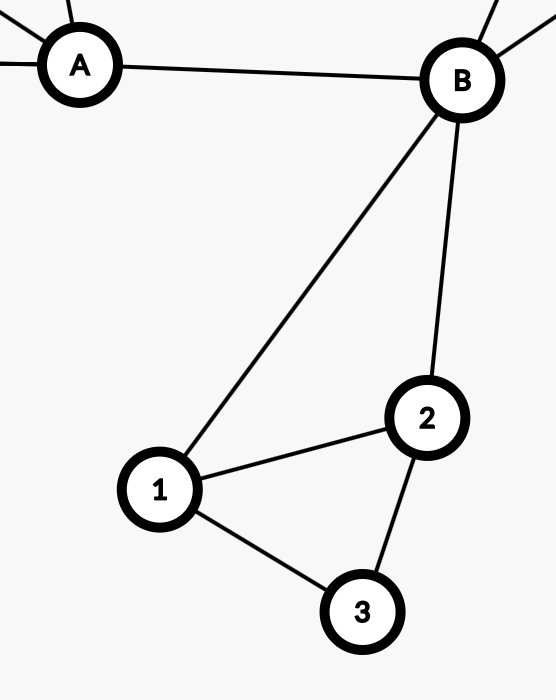
\includegraphics[width=\linewidth]{_img/340/02.png}
              \end{subfigure}
              \caption{Два возможных случая}
            \end{figure}
            Тут $\{1,2,3\}$ --- какой-то треугольник в графе $G$, а новый найденный треугольник в $G$ --- либо $\{A,1,2\}$, либо $\{B,1,2\}$.

            \item Пусть теперь из $A$ и $B$ идет в оставшуюся часть графа в совокупности меньше, чем $n - 2$ ребро. Имеем $|E'| \geq \left\lfloor\frac{{\left (n-2\right)}^2}{4}\right\rfloor - n + 2$. Удалим ребро одного из треугольников, не инцидентное $A$ или $B$. Теперь, в графе $|E| \geq \left\lfloor\frac{{\left (n-2\right)}^2}{4}\right\rfloor - n + 1$, значит, теперь в графе (по предположению индукции)~---~минимум $\left\lfloor\frac{n}{2}\right\rfloor - 1$ треугольник. Вернем ребро обратно и заметим, что оно образует недостающий треугольник, ведь удаленное ребро лежало в одном из треугольников до удаления.
        \end{enumerate}
    \end{enumerate}
\end{solution}
